%mainfile: rapport.tex

\section{Algorithme réparti}

\lstinputlisting[caption={Algorithme réparti}]{algo.txt}

\subsection{Explication de l'algorithme}
\subsubsection{Initialisation}
Lors du démarrage de l'application, la base de donnée est réconstruite. Celle-ci comporte trois bases, plus une vue :
\begin{description}
	\item[bd\_abos] contient l'ensemble des identifiants de voiture et pseudos d'utilisateur, auquel nous sommes abonnés.
	\item[bd\_offres\_abo] contient l'ensemble des identifiants de voitures, ainsi que la distance des abonnements offerts à notre portée. Cette liste comporte des priorités, nous permettant de détruire les abonnements passagers dus à un simple croisement avec un vehicule.
	\item[bd\_demandes\_abo] a un fonctionnement identique à la base d'offres, mais celui-ci intègre une partie des abonnements désirés par ces voisins.
	\item[bd\_flux] correspond à une vue des messages envoyés par nos abonnements.
\end{description}

Un timer est ensuite enclenché afin d'effectuer à interval régulier un \texttt{HeartBeat}.

\subsubsection{HeartBeat}
Ce message correspond à un battement de coeur, c'est à dire, une preuve d'existence. Ce message est diffusé à tous, mais ne pourra être relayé. Son contenu (offres et demandes du noeud et de ses voisins environnant) servira a mettre à jour les bases de données des noeuds receveurs. Ce contenu pourra alors très bien figurer dans les messages \texttt{HeartBeat} des noeuds receveur. Ce système permet de répartir la base de donnée générale des abonnements - abonnés et ceci même lorsqu'aucun message \texttt{PIE} n'est transmis.

\paragraph*{}
Afin de former ce message, il faut tout d'abord nettoyer les bases de données. La priorité de chaque offre et demande va être décrémentée, afin que les noeuds que nous ne rencontrons plus aient une priorité négative. Cette priorité pourra être calculée, uniquement sur le nombre de messages \texttt{HeartBeat} de la cible, ou en prenant en compte les coordonnées GPS de celle-ci. Au contraire, à la réception d'un message, les abonnements contenus dans les offres et les demandes verront leur priorité incrémentée.

\subsubsection{Envoi et réception d'un message PIE}
Un message PIE correspond au message que l'utilisateur veut envoyer à ses suiveurs, de la même façon que sur \texttt{Tweeter}. Ce message doit donc être acheminé jusqu'à chaque voiture concernée par celui-ci. Insérer une limite de distance dans la diffusion du message impliquerait une limite fixe, et ainsi un long convoi de voiture ne sera pas pris en compte. Augmenter la distance maximale de diffusion implique une diffusion lointaine vers des zones sans intérêt. C'est pour cela que nous avons introduit deux notions : le TTL et le TTS.

\paragraph*{}
Le TTL (Time To Live) va être décrémenté chaque fois qu'une voiture retransmet le message alors que l'abonnement ne figure pas dans sa base de donnée \texttt{bd\_demandes\_abo}.
\paragraph*{}
Le TTS (Time To Survive) va être décrémenté par chaque voiture retransmettant le message alors que l'abonnement figure dans la base de donnée \texttt{bd\_demandes\_abo}.
\paragraph*{}
Un seul de ces deux compteurs peut être décrémenté. Le message n'est pas retransmis si le compteur devant être décrémenté est à 0. Ce mode de retransmission permet une diffusion intelligente. En effet, le message peut être diffusé inutilement dans un rayon égal au TTL. Cependant, il pourra s'étendre d'avantage dans les zones où un destinataire est présent grâce au TTS. Le schéma ci-dessous montre ce principe.

\begin{center}
	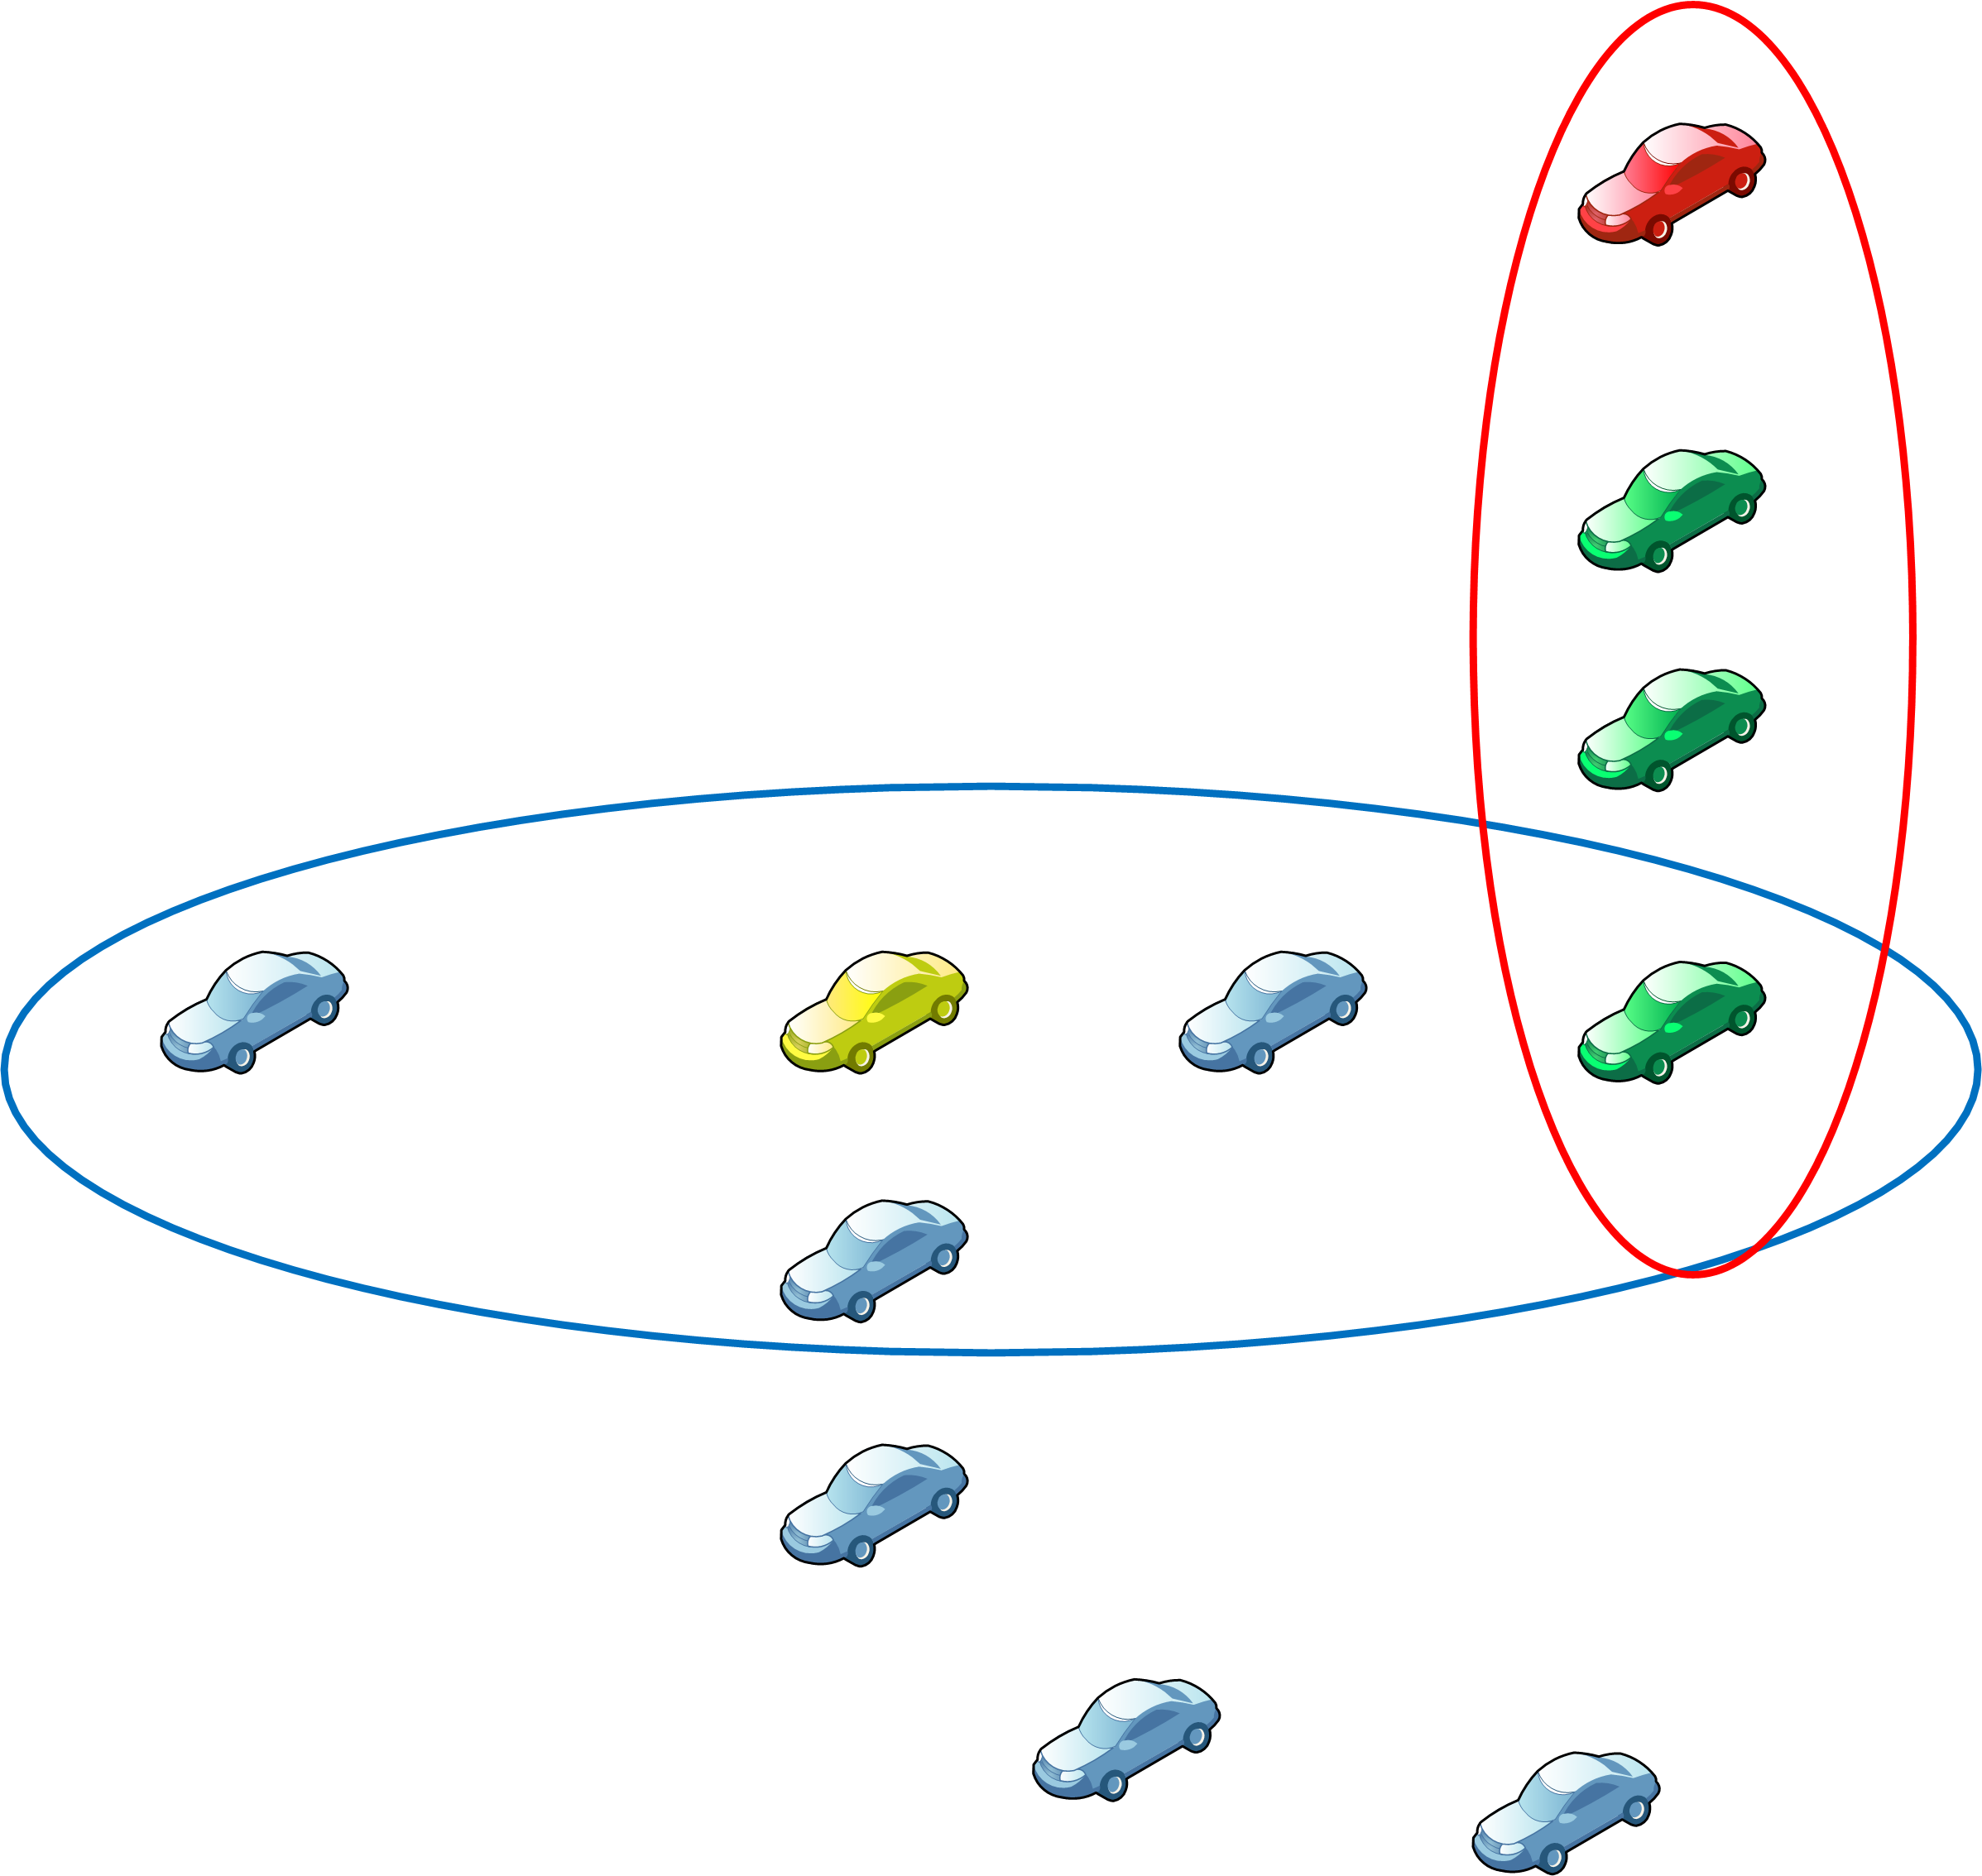
\includegraphics[width=0.75\textwidth]{img/schema2}
\end{center}

\paragraph*{}
\begin{description}
	\item[Voiture jaune :] Noeud émetteur du message PIE.
	\item[Voiture bleue :] Noeud non abonné et non intéressé par le message.
	\item[Voiture verte :] Noeud non abonné, mais connaissant un noeud intéressé par celui-ci.
	\item[Voiture rouge :] Noeud abonné à l'émetteur désirant donc recevoir le message.
	\item[Ellipse bleu :] Zone de diffusion du message par décrémentation du TTL.
	\item[Ellipse rouge :] Zone de diffusion du message par décrémentation du TTS.
\end{description}
\paragraph*{}
Nous remarquons que contrairement à une diffusion par distance qui aurait un format de cercle, l'utilisation du TTL et TTS permet une diffusion ayant une forme variable. Dans le cas d'un convoi de vehicule, avec un vehicule égaré, cela va par exemple permettre de continuer à faire communiquer les deux protagonistes le plus longtemps possible.


\paragraph*{}
Dans un soucis d'optimiser chaque message, et d'avoir une convergence rapide des bases de données, avec la topologie physique de notre réseau de voitures, nous avons choisi d'inclure les offres et les demandes aux messages \texttt{PIE}. Ainsi ces messages participeront à un meilleur acheminement des futurs messages du réseau.
